\input{boilerplate}
\begin{document}
\bibliographystyle{unsrt}

\title{High-resolution 7-Tesla fMRI data on the perception of musical genres -- an extension to the \textit{studyforrest} dataset}

\author[1,2]{Michael~Hanke}
\author[1]{Richard~Dinga}
\author[1]{Christian~Häusler}
\author[3]{J.~Swaroop~Guntupalli}
\author[1,4]{Michael~Casey}
\author[1,5]{Falko~R.~Kaule}
\author[6]{J\"org~Stadler}

\affil[1]{Psychoinformatics lab, Department of Psychology II, University of
Magdeburg, Magdeburg, Germany}
\affil[2]{Center for Behavioral Brain Sciences, Magdeburg, Germany}
\affil[3]{Department of Psychological and Brain Sciences,
  Dartmouth College, Hanover, New Hampshire, USA}
\affil[4]{Bregman Laboratory, Deptartment of Music and Deptartment of Computer
  Science, Dartmouth College, Hanover, New Hampshire, USA}
\affil[5]{Visual Processing Laboratory, Ophthalmic Department,
Otto-von-Guericke-University, Magdeburg, Germany}
\affil[6]{Leibniz Institute for Neurobiology, Magdeburg, Germany}
\maketitle
\thispagestyle{fancy}

\begin{abstract}
% Abstracts should be up to 300 words and provide a succinct summary of the
% article. Although the abstract should explain why the article might be
% interesting, care should be taken not to inappropriately over-emphasise the
% importance of the work described in the article. Citations should not be used
% in the abstract, and the use of abbreviations should be minimized.

Here we present an extension to the \textit{studyforrest} dataset -- a
versatile resource for studying the behavior of the human brain in situations
of real-life complexity (\url{http://studyforrest.org}). This release adds more
high-resolution, ultra high-field (\unit[7]{Tesla}) functional magnetic resonance
imaging (fMRI) data from the same individuals. The twenty participants were
repeatedly stimulated with a total of 25 music clips, with and without speech
content, from five different genres using a slow event-related paradigm. The
data release includes raw fMRI data, as well as pre-computed structural
alignments for within-subject and group analysis.  In addition to fMRI,
simultaneously recorded cardiac and respiratory traces, as well the complete
implementation of the stimulation paradigm, including stimuli, are provided. An
initial quality control analysis reveals distinguishable patterns of response
to individual genres throughout a large expanse of areas known to be involved
in auditory and speech processing.  The present data can be used to, for
example, generate encoding models for music perception that can be validated
against the previously released fMRI data from stimulation with the ``Forrest
Gump'' audio-movie and its rich musical content.  In order to facilitate
replicative and derived works, only free and open-source software was utilized.

\end{abstract}
\clearpage

\section*{Background}
%The format of the main body of the article is flexible: it should be concise
%and in the format most appropriate to displaying the content of the article.

%A brief summary of how this work was motivated and how it links to existing
%and future work.

Previously, we have released a large, high-resolution, \unit[7]{Tesla} fMRI
dataset on the processing of natural auditory stimuli -- a two-hour audio movie
\cite{HBI+14}.  Recently, we have extended this initial release with a detailed
annotation of the emotional content of the stimulus \cite{LRS+2015} to broaden
the range of research questions that could be addressed with these data.  Here
we further amend this dataset with additional high-resolution fMRI data from
the same participants on the perception of musical genres.  We employed a
proven paradigm and stimuli that have been previously shown to to enable
investigation of distributed population codes of musical timbre in bilateral
superior temporal cortices \cite{CTK+2012}. 

The present data release enables comparative studies of the representation of
musical genres (spectrum, timbre, vocal content) with ultra high-field, high
resolution fMRI data from a larger sample of participants. In conjuction with
the previous data releases, it will also further expand the continuum of
research question that can be approached with the joint dataset. For example, the
development of encoding models for cortical representations of music in complex
auditory stimuli (the audio-movie contains several dozen musical excerpts from
a broad range of genres).  These data can also serve as a public resource for
benchmarking algorithms for functional alignment \cite[e.g., ][]{HGC+11}, or
other analyses, and thus, further the availability of resources for the
investigation of real-life cognition \cite{HH2015}.

\section*{Materials and methods}
\subsection*{Participants}

Acquisition of the data described herein was part of a previously published
study \cite{HBI+14}, and took place in close temporal proximity (no more
than a few weeks apart). The participants in this data release are identical to
those previously reported.  They were fully instructed about
the nature of the study and were paid a total of \unit[100]{EUR} for their
participation, which included the previously reported data acquisitions, as
well as the one described herein. All data acquisitions were jointly approved
by the ethics committee of the Otto-von-Guericke-University of Magdeburg,
Germany.


\subsection*{Stimulus}

All stimuli employed in this study are identical to those used in a previous
study \cite[for details refer to][]{CTK+2012}. They were five natural,
stereo, high-quality music stimuli for each of five different musical genres:
1) Ambient, 2) Roots Country 3) Heavy Metal, 4) 50s Rock'n'Roll, and 5)
Symphonic (see Figure \ref{fig:spectrograms} for details).


\begin{figure*}
  \centering
  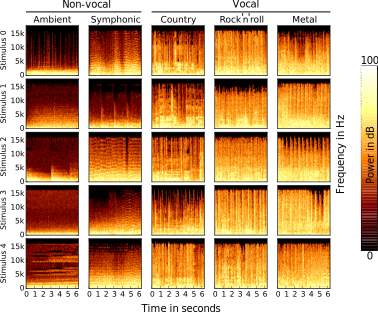
\includegraphics[width=11.5cm]{stimulus_specgrams}\\

  \caption{
    %
    Spectrograms for all 25 stimuli showing structural differences in the
    time-frequency characteristics of the five musical genres.  Each stimulus
    was a six second excerpt from the middle of a distinct musical piece.
    Excerpts were normalized so that their root-mean-square power values were
    equal, and a \unit[50]{ms} quarter-sine ramp was applied at the start and
    end of each excerpt to suppress transients.  Most prominent are the
    differences between music clips with and without vocal components.
  %
  }

  \label{fig:spectrograms}
\end{figure*}


\subsection*{Procedures and stimulation setup}

The setup for audio-visual presentation was as previously reported
\cite{HBI+14}. Participants listened to the audio using custom-built in-ear
headphones, and an LCD projector displayed visual instructions on a
rear-projection screen that they saw via a mirror attached to the head coil.

At the start of each recording session, during the preparatory MR scans,
participants listened to a series of longer excerpts of musical pieces and
songs from the five different genres. During this phase participants were
instructed to request adjustments of the stimulus volume in order to guarantee
optimal perception of the stimuli against the noise pedestal emitted by the
scanner. There was no overlap between the songs presented in this phase and those
used as stimuli in the main experiment.

Eight scanning runs followed the initial sound calibration. Each run was
started by the participant with a key-press ready signal. There were 25 trials,
with five different stimuli (Figure~\ref{fig:spectrograms}) for each of the
five genres per run (see Figure~\ref{fig:design} for details on the experiment
design). At the end of each run participants were given the opportunity for a
break of variable length until they indicated readiness for the next run. Most
participants started the next run within a minute.

\begin{figure*}[t]
  \centering
  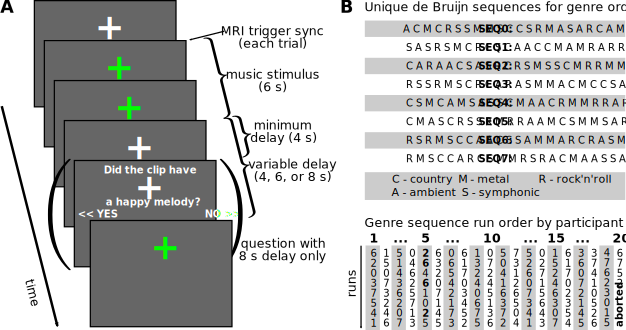
\includegraphics[width=16cm]{design}

  \caption{
  %
  Experiment design.
  %
  (A) Trial configuration. The start of each trial was synchronized with the
  MRI volume acquisition trigger. When the trigger was received the permanently
  displayed white fixation cross turned green, a \unit[6]{s} music stimulus was
  presented, and, immediately afterwards, the fixation cross turned white
  again.
  %
  Stimulation was followed by a variable delay (minimum delay \unit[4]{s}). For
  the five trials of a genre, a \unit[4]{s} and \unit[8]{s} delay occurred
  once, while the remained three trials included a \unit[6]{s} delay period.
  Thereby all trials had \unit[4-8]{s} of uniform stimulation (no audio, white
  fixation cross) after each musical stimulus.
  %
  The order of delays was randomized within a run. During trials with an
  \unit[8]{s} second delay participants were presented with a yes/no question
  four seconds after the end of the music stimulus. The content of the question
  was randomized and asked for particular features of the stimulus that had
  just ended (e.g., ``Was there a female singer?'', ``Did the song have a happy
  melody?'').  Participants had to indicate their response by pressing one of
  two buttons with the index or middle finger of their right hand corresponding
  to the response alternative presented on the screen.  ``Yes'' was always
  mapped to the left side (index finger), ``No'' always to the right side
  (middle finger).  The question had the purpose of keeping the participants
  attentive to the stimuli and counteract the effect of increasing familiarity
  across multiple runs. 
  %
  (B) Run configuration. The 25 stimuli were identical across runs and
  presented exactly once per run. Order of stimulus genres within each run was
  counter-balanced using De Bruijn cycles \cite{AMM+2011} (alphabet size = 5,
  counter-balancing level = 2), hence each genre was followed by any other
  genre equally often and exactly once.  Eight unique genre order sequences
  were generated and used for all participants, while randomizing the order of
  run sequences across participants. This was done in order to enable the
  application of the hyperalignment algorithm \cite{HGC+11}. Data acquisition
  for two participants showed anomalies with respect to this procedure (see
  Table~\ref{tab:anomalies} for details).
  %
  }

  \label{fig:design}
\end{figure*}

Stimulus presentation and response logging were implemented using PsychoPy
\cite{Pie2007}  running on a computer with the (Neuro)Debian operating system
\cite{HH12}.

\subsection*{Functional MRI data acquisition}

The acquisition protocol for functional MRI was largely identical with the one
previously reported \cite{HBI+14}, hence only differences and key facts are
listed here.

Importantly, the same landmark-based procedure for automatic slice positioning
that was used to align the scanner field-of-view between acquisition sessions,
was used again to align the field-of-view for this acquisition with the one in
the previous study \cite{HBI+14}. As the exact same alignment target was
used, this led to a very similar field-of-view configuration across
acquisitions.

Each acquisition run consisted of 153 volumes (repetition time of 2.0 seconds
with no inter-volume gaps).

\subsection*{Physiological recordings}

The cardiac and respiratory traces were recorded for the full duration of all
eight runs. The acquisition setup for physiological was identical with the one
previously reported \cite{HBI+14}.

\section*{Dataset content}

The released data comprises raw and pre-processed fMRI data, physiological
recordings, behavioral log files, and auditory stimuli (total
$\approx$\unit[95]{GB}). Table~\ref{tab:dslayout} provides an overview of the
location of individual data components. The following sections briefly describe
important properties.

\begin{table*}[p]
  \centering
  \caption{Data set layout. File paths and descriptions for all available content.}
  \begin{tabular}{p{2mm}p{65mm}p{95mm}}
    \toprule
    \multicolumn{2}{l}{\textbf{File path}} & \textbf{Description} \\
    \toprule
    \multicolumn{2}{l}{\texttt{/}} & \textbf{Meta data} \\
    & \texttt{[model,scan,study,task]\_key.txt} & OpenFMRI study meta data \\
    & \texttt{models/model001/[condition\_key,task\_contrasts].txt} & \\
    & \texttt{acquisition\_protocols/task002\_fmri\_session.pdf} \\
    & & Siemens 7T Magnetom acquisition protocol settings\\
    \midrule
    \multicolumn{2}{l}{\texttt{stimulus/task002/}} & \textbf{Stimulus file and paradigm implementation}\\
    & \texttt{[intro,runs].csv} & Helper CSV tables for PsychoPy experiment \\
    & \texttt{make\_design.py} & Script for random stimulation sequence generation \\
    & \texttt{mg\_7T.psyexp} & PsychoPy (v1.82) builder experiment implementation \\
    & \texttt{stimuli/[ambient,country,metal,rocknroll,symphonic]\_00[0-4].wav} \\
    & & Stimulus files (PCM WAVE, \unit[16]{bit}, \unit[44100]{Hz} stereo)\\

    \midrule
    \multicolumn{3}{l}{\texttt{SUBJECT/behav/task002\_run00[1-8]/behavdata.txt}} \\
    & & \textbf{Behavioral log files} (CSV format) \\
    \multicolumn{3}{l}{\texttt{SUBJECT/model/model001/onsets/task002\_run00[1-8]/cond00[1-5].txt}} \\
    & & \textbf{Stimulation timing specifications} (FSL EV3 format)\\

    \midrule
    \multicolumn{3}{l}{\texttt{SUBJECT/physio/task002\_run00[1-8]/[physio.txt.gz,conversion.log]}} \\
    & & \textbf{Physiological data} and conversion log file \\

    \midrule
    \multicolumn{2}{l}{\texttt{SUBJECT/BOLD/task002\_run00[1-8]/}} & \textbf{BOLD fMRI data}\\
    &   \texttt{bold[\_dico].nii.gz} & Raw and distortion-corrected BOLD fMRI\\
    &   \texttt{moco\_ref.nii.gz} & Motion correction reference scan \\
    &   \texttt{bold\_dico\_moco.txt}  & Motion estimates (3x translation in mm, 3x rotation in deg)\\
    &   \texttt{*dicominfo.txt} & DICOM meta data dump from MRIConvert \\
    &   \texttt{bold\_dico\_bold7Tp1\_to\_subjbold7Tp1.nii.gz} \\
    & & BOLD fMRI aligned to per-subject template (\unit[6]{DoF}; FLIRT)\\
    &   \texttt{qa/bold\_dico\_fgmask\_bold7Tp1\_to\_subjbold7Tp1.nii.gz} \\
    & & Foreground voxel mask (across time series) \\
    &   \texttt{qa/bold\_dico\_moest\_bold7Tp1\_to\_subjbold7Tp1.txt} \\
    & & Motion estimates with respect to per-subject template (MCFLIRT)\\

    \midrule
    \multicolumn{2}{l}{\texttt{SUBJECT/templates/bold7Tp1/}} & \textbf{7T BOLD fMRI per-subject template}  (all phase 1 data) \\
    &   \texttt{[head,brain,brain\_mask].nii.gz} & Average head and skull-stripped image, plus mask \\
    &   \texttt{in\_grpbold7Tp1/[head,brain\_mask].nii.gz} \\
    & & Per-subject template in group template space\\
    &   \texttt{in\_grpbold7Tp1/[subj2tmpl,tmpl2subj]\_warp.nii.gz} \\
    & & FNIRT warps from/to group BOLD template space\\
    &   \texttt{qa/fgmasks\_bold7Tp1\_to\_subjbold7Tp1.nii.gz} \\
    & & 4D image with foreground masks across all 7T BOLD fMRI acq.\\
    &   \texttt{qa/jointfgmask\_bold7Tp1\_to\_subjbold7Tp1.nii.gz} \\
    & & Intersection of above image across volumes \\
    &   \texttt{qa/jointfgbrainmask\_bold7Tp1\_to\_subjbold7Tp1.nii.gz} \\
    & & Intersection of above image with template brain mask \\
    &   \texttt{qa/lvl2/[head,head\_avgstats,aligned\_head\_samples].nii.gz} \\
    & & Last iteration template image, overlap stats, and aligned samples prior cropping \\

    \midrule
    \multicolumn{2}{l}{\texttt{templates/grpbold7Tp1/}} & \textbf{7T BOLD fMRI group template} (all phase 1 data )\\
    &   \texttt{[head,brain].nii.gz} & Average head and skull-stripped image\\
    &   \texttt{xfm/[mni2tmpl,tmpl2mni]\_12dof.mat} & Affine transformation to/from MNI152 (FLIRT)\\
    &   \texttt{in\_mni/brain\_12dof.nii.gz} & Template transformed and re-sliced into MNI152 (1mm)\\
    &   \texttt{from\_mni/MNI152\_T1\_1mm.nii.gz} & MNI152 template from FSL in group template space \\
    &   \texttt{from\_mni/avg152T1\_[brain,csf,gray,white].nii.gz} \\
    &   \texttt{from\_mni/MNI152\_T1\_1mm\_brain\_mask[\_dil].nii.gz} \\
    &   \texttt{qa/lvl4/[head,brain].nii.gz} & Template generation overlap stats, aligned samples \\
    &   \texttt{qa/lvl4/[head\_avgstats,aligned\_head\_samples].nii.gz} \\
    &   \texttt{qa/subjbold7Tp1\_to\_grpbold7Tp1/brain\_mask\_[intersection,stats].nii.gz} \\
    &   \texttt{qa/subjbold7Tp1\_to\_grpbold7Tp1/aligned\_brain\_samples.nii.gz} \\
    & & Per-subject template alignment quality control files \\
    \bottomrule
  \end{tabular}
  \label{tab:dslayout}
\end{table*}

%\subsection*{Stimulation implementation}
%
%The complete PsychoPy experiment implementation, including the script to
%generate stimulation sequences, as well as the actual stimuli are included.

\subsection*{Behavioral log files}

Log files are available as plain text files with comma-separated value markup.
All enumerations are zero-based. Each lines represents a trial. Columns for the
following information are present: order of run in sequence (\texttt{run}), ID
of trial sequence for this run (\texttt{run\_id}; see Figure
\ref{fig:design}B), fMRI volume corresponding to stimulation start (total:
\texttt{volume}, in the current run: \texttt{run\_volume}), stimulus file name
(\texttt{stim}), music genre label (\texttt{genre}), inter-stimulus interval in
seconds (\texttt{delay}), flag whether a control question with presented
(\texttt{catch}), measured asynchrony between MRI trigger and sound onset in
seconds (\texttt{sound\_soa}), and time stamp of the corresponding MRI trigger
with respect to the start of the experiment in seconds (\texttt{trigger\_ts}).

Information on the stimulus timing is also available in per-subject, per-run,
per-condition plain-text files in FSL's EV3 format: one line per stimulation
event, three columns with stimulus \texttt{onset} and \texttt{duration} (both
in seconds relative to the start of a scan), as well as a third column with an
arbitrary intensity weight that is always set to $1$.

\subsection*{fMRI data}

All functional MRI data were converted from the DICOM format into the NIfTI
format for publication using the same procedure as in \cite{HBI+14}.

fMRI data are available in three different flavours, each stored in an
individual 4D image for each run separately. Raw BOLD data are stored in
\texttt{bold.nii.gz}. While raw BOLD data are suitable for further analysis,
they suffer from severe geometric distortions. BOLD data that have been
distortion-corrected \cite{IS2012} at the scanner console are provided in
\texttt{bold\_dico.nii.gz}. In addition, distortion-corrected data that
have been anatomically aligned to a per-subject  BOLD template image
are available: \texttt{bold\_bold7Tp1\_to\_subjbold7Tp1.nii.gz}.

\subsection*{Participant motion estimates}

Head movement correction was performed with respect to a dedicated reference
scan at the start of the recording session within scanner online reconstruction
as part of the distortion correction procedure. The associated motion estimates
are provided in a whitespace-delimited 6-column text file (translation X, Y, Z
in mm, rotation around X, Y, Z in deg) with one row per fMRI volume for each
run separately.

\subsection*{Physiological recordings}

Physiological data were truncated to start with the first MRI trigger pulse and
to end one volume acquisition duration after the last trigger pulse. Data are
provided in a four-column (MRI trigger, respiratory trace, cardiac trace and
oxygen saturation), space-delimited text file for each run. A log file of the
automated conversion procedure is provided in the same directory
(conversion.log). Sampling rate for the majority of all participants is
\unit[200]{Hz} (see Table~\ref{tab:anomalies} for exceptions). 

\subsection*{Audio features}

Recent experiments have shown that audio features can be predicted via
regression models from fMRI signals to test stimulus coding hypotheses
\cite{CTK+2012,TAB+2014}.  To facilitate this activity with the current data we
extracted four audio features from the music genre stimuli. The stimulus sample
rate was \unit[44.1]{kHz}, stereo, with duration 6s. Audio was down-mixed to
mono and feature extraction used a front-end windowed short-time Fourier
transform, with window size 16384 samples (\unit[371.52]{ms}) and hop size 4410
samples (\unit[100]{ms}) yielding 63 overlapping feature vectors per stimulus
file.  Window parameters were chosen to trade temporal for spectral acuity,
yielding frequency samples spaced linearly at \unit[2.69]{Hz} intervals from
\unit[0-22.05]{kHz}. The four features extracted from this representation are
described below and are illustrated in the audiofeatures.py reference
implementation included with task002.

\paragraph{Mel-Frequency Spectrum (mfs) -- 48 dimensions}
%
Motivated by human auditory perception the mel scale organizes frequency by
equidistant pitch locations as determined by psychophysical experiments. We
used the essentia open source audio processing library \cite{BWG+2013} to
extract the mel-frequency spectrum, which yielded energy in mel bands by
applying a frequency-domain filterbank \cite{GFK2005} to the short-time Fourier
spectrum.  Frequency-domain filtering consisted of applying equal area
overlapping triangular filters to the Fourier spectrum spaced according to the
mel scale and normalized such that the sum of coefficients for every filter
equals one.

\paragraph{Mel-Frequency Cepstral Coefficients (mfcc) -- 48 dimensions}
%
Cepstral features have been widely reported to perform well in speech
recognition and music classification systems \cite{LS2001}, where the task is
required to be sensitive to timbre.  Typically, only the lower 10-20 cepstral
coefficients (low quefrency) are retained; these encode the shape of the broad
spectral envelope -- an acoustic correlate of timbre.  However, when
sensitivity to timbre is not required, utilizing the upper coefficients (high
quefrency), that encode fine spectral structure such as pitch, makes the
feature robust to timbral changes \cite{MEK2009}. We extracted the full set of
48 cepstral coefficients from the mel-frequency spectrum, by mapping the mel
spectrum to a decibel amplitude scale and multiplying by the discrete cosine
transform (DCT-II) matrix. It is expected that any application would first
remove the constant first column and retain either the +subsequent 13-20
coefficients or the remaining upper coefficients after those, depending on
whether sensitivity or robustness to timbral difference is required. The
remaining +two features yield such a separation into low and high quefrency
spectral components.

\paragraph{Low-Quefrency and High-Quefrency Mel-Frequency Spectrum (lq\_mfs,
hq\_mfs)}
%
Although proven to be useful in machine classification tasks, cepstral
coefficients are in a different domain than the spectrum. The last two features
map selected cepstral coefficients back to the spectrum domain by
reconstructing the 48 mel-frequency spectrum bands using the low-quefrency and
high-quefrency mfcc coefficients respectively. In each case, the non-selected
coefficients were zeroed and the resulting feature mapped back to the spectral
domain using the inverse (transposed) DCT-II matrix and then inverting the
decibel amplitude scale. These two sets of features represent broad-spectrum
information (timbre) and fine-scale spectral structure (pitch) respectively.
The product of these two spectra yields the mel-frequency spectrum.

Taken together, these audio features represent the time-frequency information
of each stimulus in four different views. The views are mapped to different
perceptually-motivated scales (mel and decibel scales) and via a decorrelating
linear transformation (DCT-II). It is hoped that providing these example
features will catalyze discoveries of auditory stimulus codes in neural
populations.

\subsection*{Source code}

The source code for descriptive statistics in
figures~\ref{fig:spectrograms}~and~\ref{fig:motionqc}, as well as the
implementation for the analysis presented in figure \ref{fig:blobs} is
available in a Git repository at
\url{https://github.com/psychoinformatics-de/pandora_data}.  Source code for
the implementation of the stimulation paradigm are included in the data
release.  Additional scripts for data conversion and quality control are
available at: \url{https://github.com/hanke/gumpdata}.

\section*{Dataset validation}
%Use section and subsection commands to organize your document. \LaTeX{}
%handles all the formatting and numbering automatically. Use ref and label
%commands for cross-references.

%This section is not essential for Web Tool papers.
%For Data Articles, no analysis of the data, results or conclusions should be
%included and so this section should not be completed.

In order to assess data quality, we investigated whether different BOLD
response patterns associated with the five musical genres could be
discriminated, using either univariate statistical parametric mapping or
multivariate pattern (MVP) classification accuracy (searchlight-based analysis,
radius of two voxels, sparse spatial sampling with sphere-centers spaced by two
voxels, leave-one-run-out cross-validated classification analysis with a
support vector machine, accuracy mapped on a voxel reflects the average across
all sphere-analysis a voxel participated in).  Inspection of the participant
motion estimates revealed a median translation of less than a voxel size, and a
maximum rotation of about \unit[1]{deg} (see Figure~\ref{fig:motionqc} for
outliers). Despite the variable magnitude of motion, no participant was
excluded from the subsequent analysis.

\begin{figure*}
  \centering
  \includegraphics[width=\linewidth]{motionqc}\\
  \caption{Summary statistics for head movement estimates across runs
    and participants.
   These estimates indicate relative motion with respect to a dedicated reference scan
   at the beginning of each scan session. The area shaded in light gray depicts
   the range across participants, while the medium gray area indicates the 50\%
   percentile around the mean, and the dark gray area shows $\pm$ one
   standard error of the mean. The black line indicates the median estimate.
   Dashed vertical lines indicate run boundaries where participants had a brief
   break. The red lines indicate motion estimate time series of outlier
   participants. An outlier was defined as a participant whose motion estimate
   exceeded a distance of two standard deviations from the mean across
   participants for at least one fMRI volume in a run. For a breakdown of
   detected outliers see table \ref{tab:anomalies}.}
  \label{fig:motionqc}
\end{figure*}

The results of the univariate analysis (Figure~\ref{fig:blobs}A) and the MVP
analysis (Figure~\ref{fig:blobs}B) and Table~\ref{tab:grpsl}) identify largely
congruent areas. MVP analysis generally detects larger and more numerous areas,
either due to higher sensitivity or a comparably more liberal statistical
threshold. Noteably, clusters of above-chance classification accuracy not only
contain auditory cortex and other cortical fields related to speech and music
processing, but also the sub-cortical bilateral medial geniculate bodies, a
neural relay station immediately prior to the primary auditory cortex in the
auditory pathway \cite{KSR+2005}.

\begin{figure*}[t] \centering 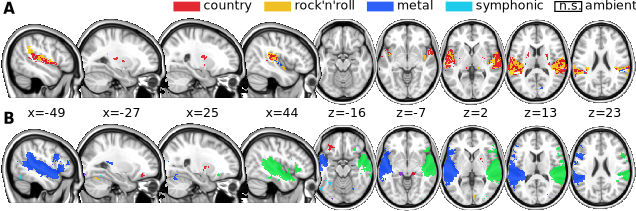
\includegraphics[width=\linewidth]{blobs}\\
  \caption{Localization of genre-discriminating signals in the brain.  (A)
    Voxel-wise genre-selectivity label. Random-effects GLM group analysis
    (n=20) were computed using the FEAT component of FSL \cite{SJW+2004}.
    Individual contrasts were evaluated for each genre to identify voxels
    showing a BOLD to this particular genre that is larger than the average
    response to all other genres. For all voxel clusters that show a
    significant difference at the group-level (cluster forming threshold
    $Z$=3.1, cluster probability threshold $p$<0.05) for any genre, the
    selectivity label was determined by the maximum $Z$ statistic across all
    genres. No significant selective activation was found for the
    \textit{ambient} genre. The majority of all voxels were labeled selective
    for one of the musical genres where stimuli contained vocals (country,
    rock'n'roll, heavy metal). Only a small cluster in BA44 R (Broca's area)
    was labeled selective for \textit{symphonic} music, despite the lack of
    speech content in these stimuli.
  %
  (B) For comparison, the location of voxel clusters with above-chance
  classification accuracy for predicting the genre of a music stimulus (colors
  only indicate individual clusters, not association with particular genres).
  The associated areas are largely
  overlapping with the results of the GLM analysis. However,
  genre-discriminating signals were identified in a number of additional areas.
  For details on the MVP analysis and cluster statistics see
  Table~\ref{tab:grpsl}. Unthresholded maps for GLM and MVP analyses are
  available at NeuroVault.org \cite{GVR+2015} \href{http://neurovault.org/collections/308/}{collection 308}.}
  %
  \label{fig:blobs} \end{figure*}

Given the confirmed wide-spread availability of genre-discriminating signal
we conclude that these data are suitable for studying the representation of
music and auditory features. Table~\ref{tab:anomalies} contains a list of all
known data anomalies that may help potential data consumers to select
appropriate subsets of this dataset.


\begin{table*}[t]
  \centering
  \caption{Overview of known data anomalies (F: functional data,
    P: physiological recordings during fMRI session)}
    \resizebox{\linewidth}{!}{\renewcommand{\arraystretch}{1.2}
  \begin{tabular}{lllp{12cm}}
    \toprule
    Modality & Participant & Run & Description \\
    \midrule
    P & 1,2 & 1-8 & sampling rate is \unit[100]{Hz} \\
    F & 2 & 2 & significant movement (translation) during scan \\
    F & 5 & 3,7 & experiment had to be restarted after the second run; due to technical limitations sequences for the first two runs were repeated as run 4 and 7 (see Figure~\ref{fig:design}B) \\
    F & 5 & 4-7 & significant movement (rotation) during scan \\
    F & 8 & 6-8 & significant movement (rotation) during scan \\
    F & 10 & 5-7 & significant movement during scan \\
    F & 11 & 4-8 & significant movement (translation) during scan \\
    F & 13 & 7-8 & significant movement (translation) during scan \\
    P & 18 & 6 & accidental data acquisition stop during the run \\
    F & 19 & 3-4 & significant movement (translation) during scan \\
    F & 20 & 2 & significant movement (translation) during scan \\
    F \& P & 20 & 5-8 & no data; participant aborted experiment after four runs \\
    \bottomrule
  \end{tabular}
}
  \label{tab:anomalies}
\end{table*}


\begin{table*}[t]
  \centering
  \resizebox{\linewidth}{!}{%
  \begin{tabular}{rrrrrrrrrrrrp{3cm}}
\toprule 
& & & \multicolumn{3}{r}{max location (MNI)} & & & \multicolumn{3}{r}{center of mass (MNI)} & \\ \cmidrule{4-6} \cmidrule{9-11}
\# & voxels & max & X & Y & Z & mean & std & X & Y & Z & $p_{corr.}$ & structure \\
\midrule
1 & 36099 & 0.53 & -58.0 & -3.9 & -0.1 & 0.31 & 0.071 & -52.1 & -20.2 & 4.7 & 0.0006 & L sup.~temporal, L Broca's area, L front.~operculum \\
2 & 34451 & 0.52 & 59.5 & 0.0 & -5.4 & 0.31 & 0.071 & 53.9 & -17.8 & 1.7 & 0.0006 &  R sup.~temporal, R Broca's area, R front.~operculum \\
3 & 320 & 0.26 & -26.5 & 32.5 & -14.5 & 0.24 & 0.008 & -29.9 & 32.3 & -15.7 & 0.0142 & L front.~orbital \\
4 & 259 & 0.25 & -24.8 & -66.3 & -19.4 & 0.24 & 0.007 & -22.7 & -65.5 & -20.6 & 0.0142 & L cerebellum \\
5 & 240 & 0.25 & -40.7 & -45.0 & -16.8 & 0.24 & 0.005 & -35.3 & -51.7 & -16.6 & 0.0142 & L temporal occ. fusiform \\
6 & 227 & 0.27 & 28.0 & -63.2 & -22.7 & 0.24 & 0.007 & 25.3 & -64.2 & -18.1 & 0.0142 & R cerebullum, R temp. occ. fusiform\\
7 & 227 & 0.26 & 33.5 & -86.9 & -3.1 & 0.24 & 0.005 & 33.6 & -88.5 & -0.3 & 0.0142 & R lat. occipital\\
8 & 215 & 0.28 & 14.4 & -30.3 & -4.2 & 0.25 & 0.011 & 14.8 & -29.9 & -6.4 & 0.0145 & R medial geniculate body \\
9 & 200 & 0.28 & -13.2 & -31.0 & -7.8 & 0.24 & 0.011 & -14.1 & -30.5 & -6.6 & 0.0159 & L medial geniculate body \\
10 & 178 & 0.26 & -50.0 & -63.1 & -19.4 & 0.24 & 0.011 & -51.0 & -64.4 & -18.3 & 0.0194 & L temporooccipital \\
11 & 152 & 0.25 & 31.1 & -79.1 & 9.3 & 0.24 & 0.004 & 32.6 & -79.0 & 9.6 & 0.0268 & R lat. occipital \\
12 & 144 & 0.27 & 28.8 & 28.7 & -14.8 & 0.25 & 0.007 & 27.4 & 27.7 & -14.5 & 0.0280 & R front. orbital \\
13 & 124 & 0.25 & 24.8 & -1.2 & 4.0 & 0.24 & 0.003 & 23.2 & 0.4 & 3.2 & 0.0387 & R putamen \\
14 & 111 & 0.25 & -25.5 & -89.8 & -15.2 & 0.24 & 0.006 & -26.2 & -90.0 & -13.2 & 0.0477 & L V4 \\
15 & 107 & 0.25 & 7.1 & -83.4 & 3.3 & 0.24 & 0.005 & 6.4 & -86.1 & 1.8 & 0.0488 & R V1\\

\bottomrule
\end{tabular}
}%resize

  \caption{
  %
    Average group results of a searchlight-based (radius
    $\approx$\unit[2.5]{mm}) cross-validated within-subject musical genre
    classification analysis (n=20; SVM classifier; $C$ parameter scaled
    according to the norm of the data). The table lists statistics (size,
    mean/max/std accuracy) as well as localization information (coordinates in
    mm MNI152) for clusters with above-chance classification performance in the
    group (cluster-level probability $p$<0.05; FWE-corrected). Clusters are
    depicted in Figure~\ref{fig:blobs}B. Statistical
    evaluation was implemented using a bootstrapped permutation analysis, as
    described by Stelzer and colleagues \cite{SCT2013} and implemented in
    PyMVPA \cite{HHS09b}, using 50 permutation searchlight accuracy maps per
    subject, 10000 bootstrap samples, voxel-wise cluster forming threshold of
    $p$<0.001).
  %
  Apart from two large clusters covering the majority of bilateral area for
  auditory perception and speech processing, additional clusters with
  genre-discrimitating signals were identified. These include the bilateral
  medial geniculate bodys, as well as smaller regions on the ventral visual
  pathway, frontal orbital cortex, and the cerebellum. For these regions the
  NeuroSynth database \cite{YPN+2011} reports high posterior probabilities for
  the topics: \textit{counting, motor, naming, phonology, prosody, visual, and
  vocal} (as determined with the Neurosynth term atlas shipped with NeuroDebian
  \cite{HH12}).  }

  \label{tab:grpsl}
\end{table*}



\section*{Usage notes}

These data are part of a larger public dataset available at
\url{http://www.studyforrest.org}. The website includes information on all
available resources, data access options, publications that employ this
dataset, as well as source code for data conversion and data processing.

All data are made available under the terms of the Public Domain Dedication and
License (PDDL; \url{http://opendatacommons.org/licenses/pddl/1.0/}). All source
code is released under the terms of the MIT license
(\url{http://www.opensource.org/licenses/MIT}). In short, this means that
anybody is free to download and use this dataset for any purpose as well as to
produce and re-share derived data artifacts. While not legally required, we
hope that all users of the data will acknowledge the original authors by citing
this publication and follow good scientific practice as laid out in the ODC
Attribution/Share-Alike Community Norms
(\url{http://opendatacommons.org/norms/odc-by-sa/}).

\section*{Data availability}
\texttt{This section will be generated.}

\section*{Consent}

Written informed consent for publication of acquired data in a de-identified
form was obtained from all participants.

\section*{Author contributions}
%In order to give appropriate credit to each author of an article, the
%individual contributions of each author to the manuscript should be detailed
%in this section. We recommend using author initials and then stating briefly
%how they contributed.

MH conducted the study, implemented the stimulation paradigm, performed dataset validation analysis, and wrote the manuscript.
RD implemented and performed the dataset validation analyses.
CH converted the stimulation protocol into the OpenFMRI format.
JSG contributed to the implementation of the stimulation paradigm, and contributed to the validation analysis.
MC contributed the stimuli.
FRK contributed to quality control analysis and to the manuscript.
JS was the data acquisition lead.

\section*{Competing Interests}
No competing interests were disclosed.

\section*{Grant Information}

This research was supported by the German Federal Ministry of Education and
Research (BMBF) as part of a US-German collaboration in computational
neuroscience (CRCNS; awarded to James Haxby, Peter Ramadge, and Michael Hanke),
co-funded by the BMBF and the US National Science Foundation (BMBF 01GQ1112;
NSF 1129855). Work on the data-sharing technology employed for this research
was supported by US-German CRCNS project awarded to Yaroslav~O.~Halchenko and
Michael Hanke, co-funded by the BMBF and the US National Science Foundation
(BMBF 01GQ1411; NSF 1429999).  Michael Hanke was supported by funds from the
German federal state of Saxony-Anhalt, Project: Center for Behavioral Brain
Sciences.

\section*{Acknowledgements}
%This section should acknowledge anyone who contributed to the research or the
%article but who does not qualify as an author based on the criteria provided
%earlier (e.g. someone or an organisation that provided writing assistance).
%Please state how they contributed; authors should obtain permission to
%acknowledge from all those mentioned in the Acknowledgements section.  Please
%do not list grant funding in this section (this should be included in the
%Grant information section - See above).

We are grateful to Stefan Pollmann and Andr\'e Brechmann for their feedback on
the results of the classification analysis.
%
We acknowledge the support of the Combinatorial NeuroImaging Core
Facility at the Leibniz Institute for Neurobiology in Magdeburg.
%
Only open-source software was employed in this study. We thank their respective
authors for making it publicly available.

\newpage
\bibliography{references}

\end{document}

% vim: textwidth=80 colorcolumn=81
